\section{Additional Details to Err. Analysis \S\ref{sec:app_err_analysis}}
\label{appendix:err_analysis}

\subsection{Additional Case Study: Quantifiers}
\label{appendix:err_analysis_quantifier_case}

\begin{figure}[t]
\centering
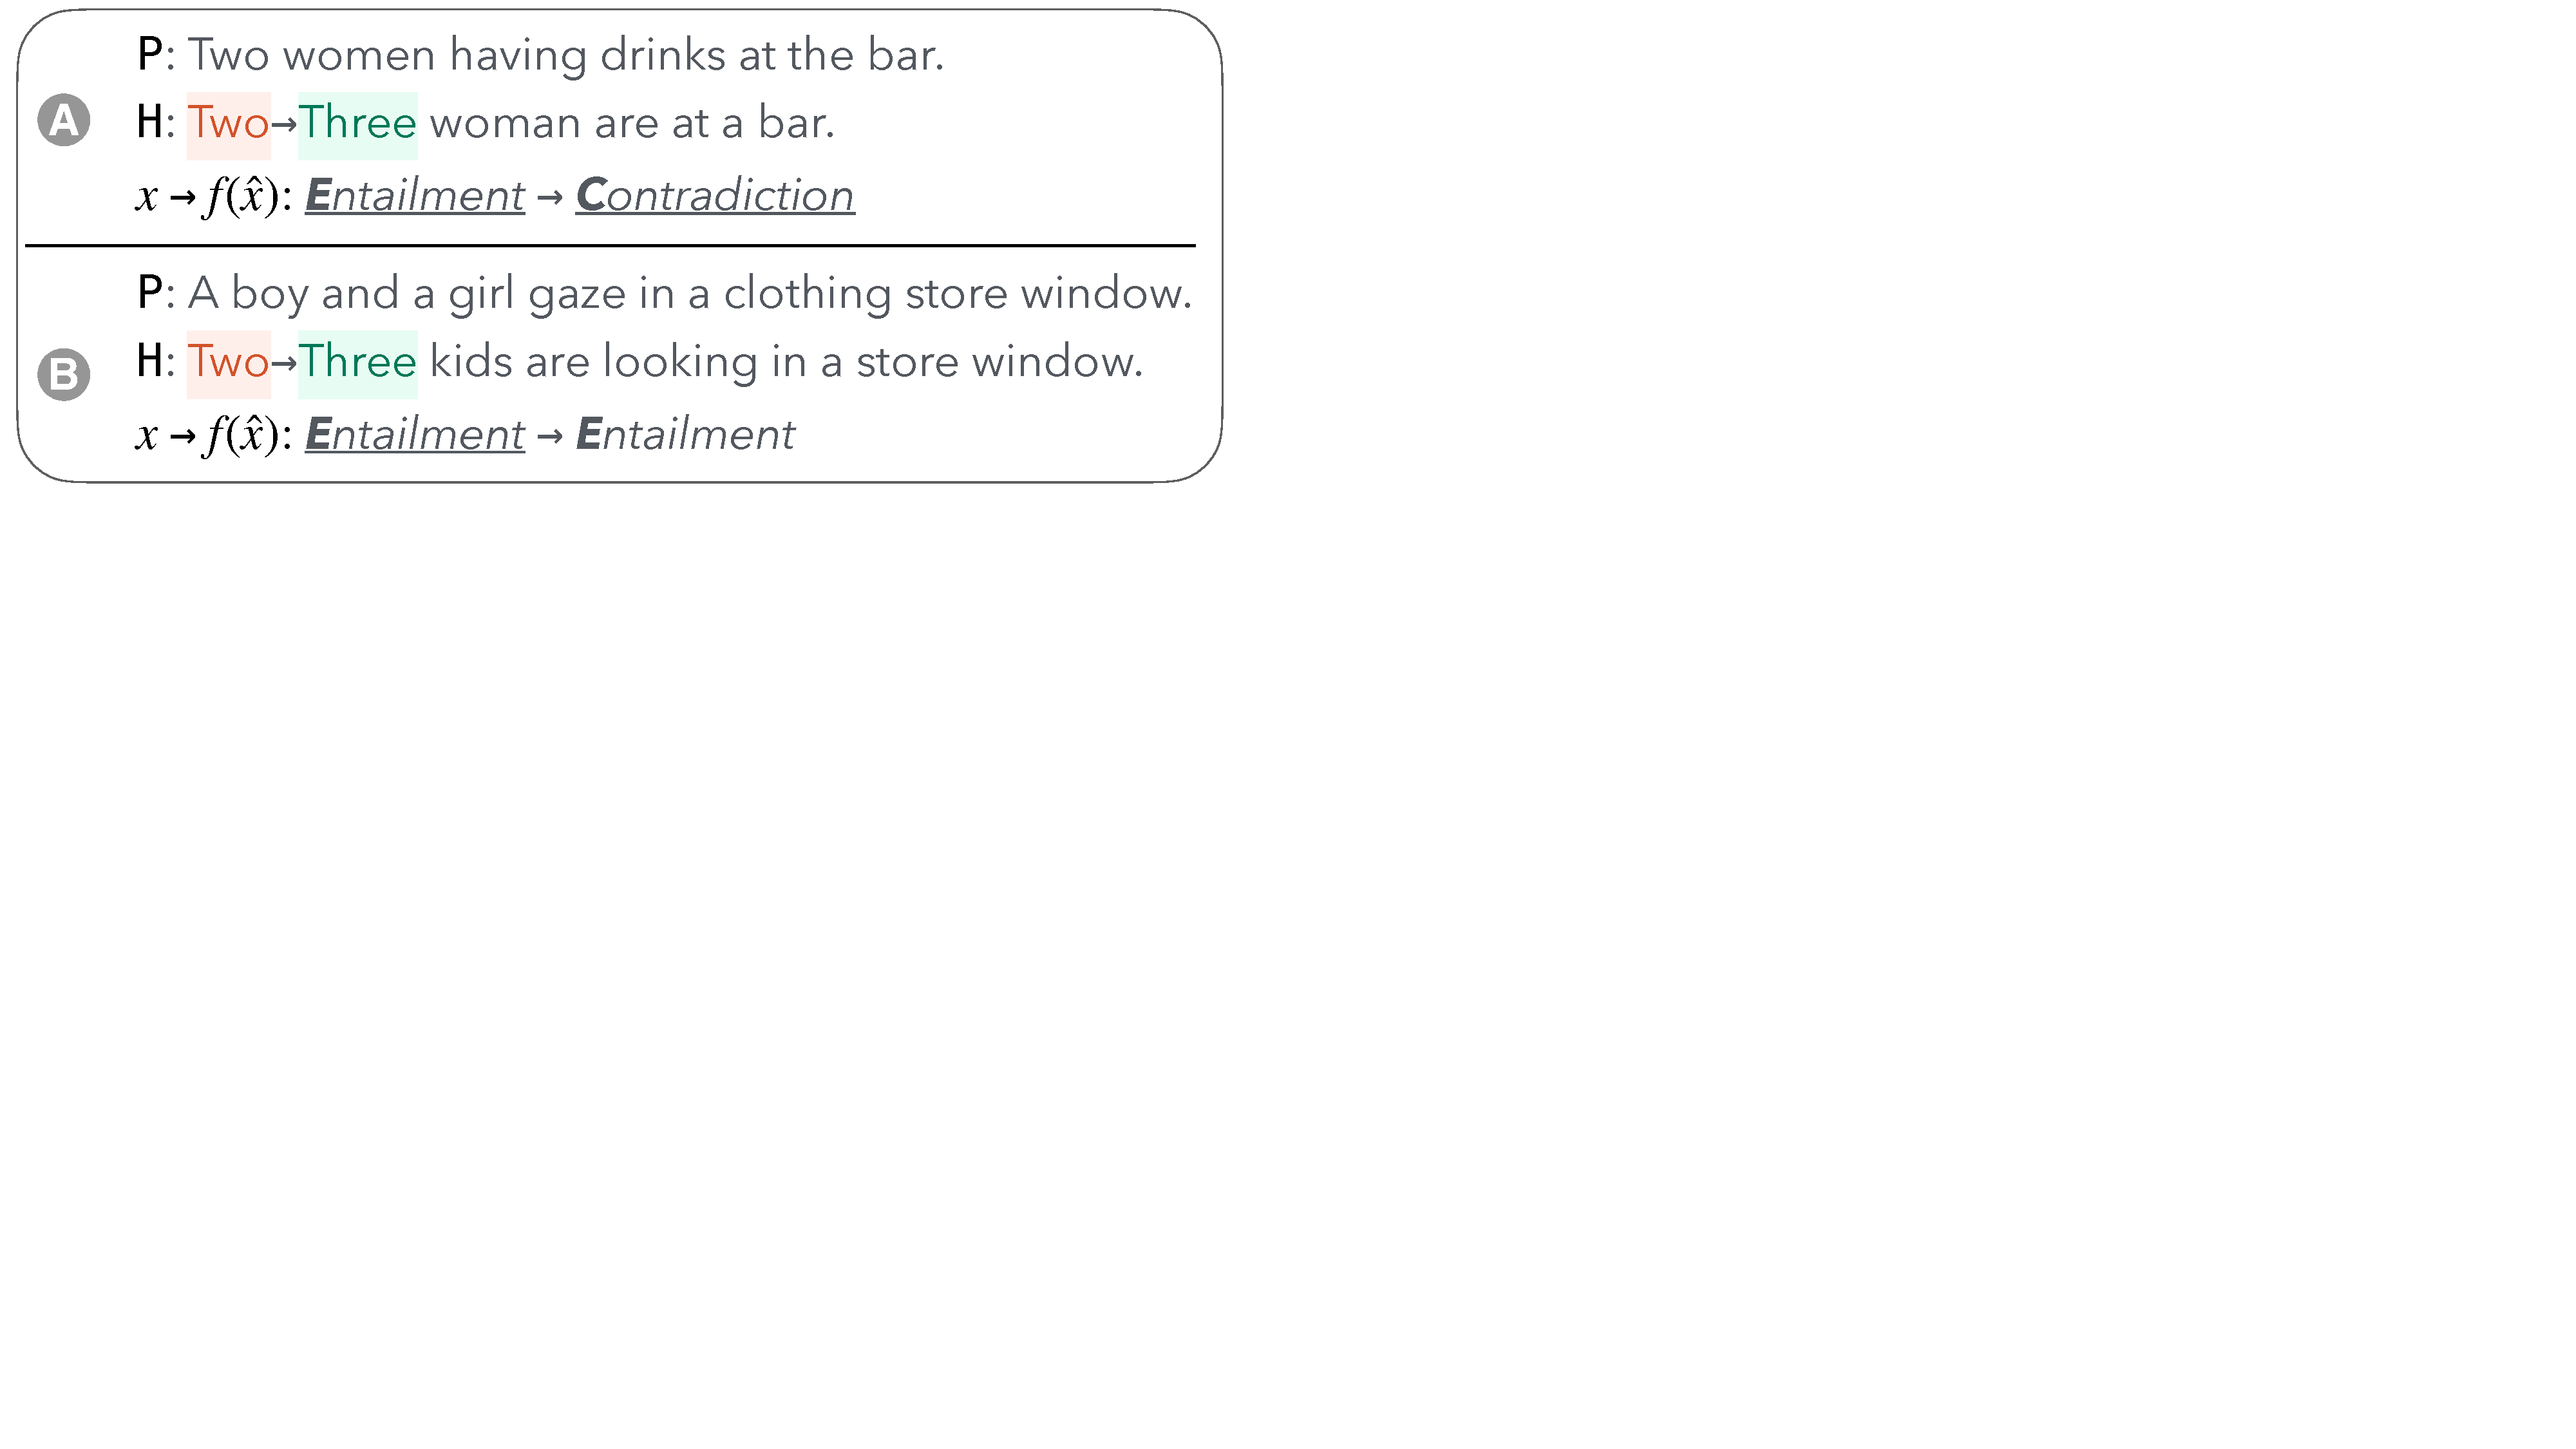
\includegraphics[trim={0 25.2cm 34.5cm 0cm},clip,width=1\columnwidth]{figures/err_analysis_two_three}
\vspace{-15pt}
\caption{
The \nli model cannot perform the actual counting when the exact number is missing from \emph{P}.
In (B), it still predicts (the now incorrect) \emph{Entailment}.
}
\vspace{-10pt}
\label{fig:err_analysis_two_three}
\end{figure}


%\citet{gururangan2018annotation} also mentioned that one common strategy for creating NLI examples is to modify the numbers, suggesting that the model should have seen various examples related to numbers.

As a follow up to the case in Figure~\ref{fig:err_analysis_quantifier}, we slice the data to find \emph{entailement} instances that have numbers in the hypothesis sentence, and perform \ctrltag{quantifier} changes on them.
Through the extracted templates, we notice two things: 
First, the model does not perform actual counting. 
When changing one number to another (\swap{\texttt{NUM}}{\texttt{NUM}}), the model only flips the label in 64.7\% cases, which is abnormal --- we would expect all cases to be like in Figure~\ref{fig:err_analysis_two_three}.
Diving into the instances, we realize that the model can be easily confused when the explicit number is not in the premise. Indeed, when we further filter the instance to only keep instances like in Figure~\ref{fig:err_analysis_two_three}B, the label flip rate of \swap{\texttt{NUM}}{\texttt{NUM}} further decreases to 30.2\%.


Second, the model can react to \emph{some} quantifier phrase modifiers. 
\swap{}{at least} (\exinline{\add{at least} women are at a bar}) will always still result in \emph{entailment}, prediction, \swap{}{only} and \swap{}{exactly} flip the predicted label to \emph{neutral} 90\% of the time (\exinline{\add{exactly} women are at a bar}), but the model only changes the prediction 52.6\% of the time when we add \swap{}{more than} (\exinline{\add{more than} women are at a bar}).


\subsection{Representative Perturbation Templates}
\label{appendix:err_analysis_template}

Similar to \citet{wu2020tempura}, the process of finding representative perturbation patterns take two steps:

\paragraph{Extract template.}
For each counterfacual $\xp$, we compare it with its original instance $x$, and translate the perturbed spans into templates using different combinations of the texts, the lemmas or the part-of-speech tags, optionally including surrounding contexts determined by the parsing tree structure (tokens that share the same parents as the perturbed span). 
For example \exinline{is\add{not} wearing} can be translated into a set of templates $t$ that are as finer-grained as \swap{is wearing}{is not wearing}, or as sparse as \swap{}{\texttt{PART}}.
Similarly, \exinline{is\add{not} reading} also results in \swap{}{\texttt{PART}} or \swap{}{\texttt{not}}, but not \swap{is wearing}{is not wearing}.
As such, the counterfactuals and templates form a many-to-many relationship: each query generates multiple templates, and each template covers a different group of counterfactuals.

\paragraph{Select Representative Templates.}
To support viewing representative changes among counterfactuals, we prefer (1) templates with high coverage (the number of
\emph{counterfactuals} covered by the template).
Meanwhile, to avoid overfitting to one instance (\eg extracting a template \swap{red}{\texttt{ADJ}} only because the word ``red'' is repeated perturbed in one $x$, which produces 100 $\xp$), we want to (3) prioritize templates that perturb a variety of unique original $x$.
We also prefer finer-grained templates, to avoid being unnecessarily abstract (\eg it is unnecessary to further abstract ``not'' if it is the only \texttt{PART} changed.)

%$\hat{\xset}_i$

With these intuitions, we form the template selection as a weighted set coverage problem.
We see the counterfactual set $\hat{\xset} = \{\xp_1,...,\xp_n\}$, the union of counterfactuals for each $x$, as the entire set of elements.
Then, each template $t \in T = {t_1,...,t_m}$ represents a subset of $\hat{\xset}$ that contains a number of counterfactuals $|t|$.
We define the weight as $w(t) = |t|_x / g(t)$, where $|t|_x$ quantifies the unique original $x$ covered by $t$, and $g(t)$ represents the heuristic weights of $t$ (increases from \texttt{LEMMA}, \texttt{TAG} to \texttt{POS}).
In this way, templates that are too abstract or too focused on a certain $x$ are penalized by having a high weight. Our goal is to find a set $T^* \subset T$ such that (1) $T^*$ with a specific size $n$; and
%(2) the sum of the weights of the subsets in $T^∗$ is minimized.
We use a classic greedy algorithm to compute an approximate $T^*$~\cite{vazirani2013approximation}.
